\subsection{Массосохраняющая постановка кавитации (JFO)}

%% Блок 1: Вводный абзац
В подразделе~2.3.1 введены кавитационное давление~$p_{\mathrm{cav}}$
и степень заполнения~$\vartheta \in (0,\,1]$.  Цель настоящего раздела --
записать замкнутую систему уравнений для двух искомых переменных:
давления $p(x_1, x_2, t)$ и степени заполнения
$\vartheta(x_1, x_2, t)$, удовлетворяющую требованиям~1-4,
сформулированным в подразделе~2.3.1.  Толщина зазора
$h(x_1, x_2, t)$ считается заданной (суперпозиция из
подраздела~2.2.1).

%% Блок 2: Модифицированное уравнение неразрывности
В кавитационной зоне зазор заполнен жидкостью лишь частично,
поэтому эффективная толщина жидкого слоя равна~$\vartheta\,h$.
Подстановка этой величины в уравнение неразрывности приводит
к модифицированному уравнению Рейнольдса (уравнение JFO):
\begin{equation}\label{eq:jfo_conservation}
  \frac{\partial (\vartheta\,h)}{\partial t}
  + \nabla \cdot \!\left(
    -\,\frac{h^3}{12\mu}\,\nabla p
    + \frac{\vartheta\,h}{2}\,\mathbf{U}
  \right) = 0.
\end{equation}

Первое слагаемое в дивергенции представляет собой пуазейлевский
(напорный) поток, пропорциональный градиенту давления~$\nabla p$.
Второе слагаемое -- куэттовский (переносной) поток, обусловленный
движением поверхности со скоростью~$\mathbf{U}$.  При $\vartheta = 1$
уравнение~\eqref{eq:jfo_conservation} сводится к классическому
уравнению Рейнольдса.  Здесь операторы $\nabla$ и $\nabla\!\cdot$
понимаются в поверхностных координатах, соответствующих выбранной
постановке (подраздел~2.1.6).  Множитель~$\vartheta$ входит в член
накопления и в куэттовский поток.  В кавитационной зоне
$p = p_{\mathrm{cav}}$, поэтому $\nabla p = 0$ и напорный поток
отсутствует автоматически.

Принципиальное отличие постановки JFO от упрощённых моделей кавитации состоит в~следующем. В~модели Гюмбеля отрицательные давления просто обнуляются: $p := \max(p,\, p_{\mathrm{cav}})$ без какого-либо уравнения для кавитационной зоны. Это нарушает баланс масс: куэттовский поток в~зону кавитации не~компенсируется потоком из~неё, и~расход жидкости через замкнутый контур оказывается ненулевым. Следствием является систематическое завышение несущей способности по сравнению с~более точными расчётами, что подтверждается экспериментально: при высоких числах Зоммерфельда отклонение может достигать десятков процентов.

В~постановке JFO вместо простого обнуления давления вводится степень заполнения~$\vartheta$, которая описывает долю объёма зазора, занятую жидкостью. В~зоне полного заполнения $\vartheta = 1$ и~уравнение~\eqref{eq:jfo_conservation} совпадает с~классическим уравнением Рейнольдса. В~кавитационной зоне $p = p_{\mathrm{cav}}$ и~$\vartheta < 1$: жидкость и~газовые пузырьки сосуществуют в~зазоре, причём их~относительные доли изменяются так, чтобы выполнялся баланс масс. Именно введение~$\vartheta$ позволяет разрешить противоречие: давление не~опускается ниже~$p_{\mathrm{cav}}$, а~массовый баланс при~этом сохраняется.

Принципиальное отличие постановки JFO от упрощённых моделей кавитации состоит в~следующем. В~модели Гюмбеля отрицательные давления просто обнуляются: $p := \max(p,\, p_{\mathrm{cav}})$ без какого-либо уравнения для кавитационной зоны. Это нарушает баланс масс: куэттовский поток в~зону кавитации не~компенсируется потоком из~неё, и~расход жидкости через замкнутый контур оказывается ненулевым. Следствием является систематическое завышение несущей способности по сравнению с~более точными расчётами, что подтверждается экспериментально: при высоких числах Зоммерфельда отклонение может достигать десятков процентов.

В~постановке JFO вместо простого обнуления давления вводится степень заполнения~$\vartheta$, которая описывает долю объёма зазора, занятую жидкостью. В~зоне полного заполнения $\vartheta = 1$ и~уравнение~\eqref{eq:jfo_conservation} совпадает с~классическим уравнением Рейнольдса. В~кавитационной зоне $p = p_{\mathrm{cav}}$ и~$\vartheta < 1$: жидкость и~газовые пузырьки сосуществуют в~зазоре, причём их~относительные доли изменяются так, чтобы выполнялся баланс масс. Именно введение~$\vartheta$ позволяет разрешить противоречие: давление не~опускается ниже~$p_{\mathrm{cav}}$, а~массовый баланс при~этом сохраняется.

%% Блок 3: Условия комплементарности
Разделение расчётной области на зону полного заполнения и зону
кавитации определяется условиями комплементарности:
\begin{equation}\label{eq:jfo_complementarity}
  \begin{aligned}
    &p - p_{\mathrm{cav}} \geq 0, \\
    &0 \leq \vartheta \leq 1, \\
    &(p - p_{\mathrm{cav}})\,(1 - \vartheta) = 0.
  \end{aligned}
\end{equation}

Из этих условий следует: либо $p > p_{\mathrm{cav}}$ и тогда
$\vartheta = 1$ (полное заполнение), либо $\vartheta < 1$ и тогда
$p = p_{\mathrm{cav}}$ (кавитация).  Промежуточные состояния
($p > p_{\mathrm{cav}}$ и одновременно $\vartheta < 1$) исключены.
Вместе с уравнением~\eqref{eq:jfo_conservation}
условия~\eqref{eq:jfo_complementarity} образуют замкнутую задачу
для двух неизвестных~$p$ и~$\vartheta$.

Задача~\eqref{eq:jfo_conservation}--\eqref{eq:jfo_complementarity} относится к~классу задач со~свободными границами. Граница разрыва плёнки~-- линия, на~которой $\vartheta$ убывает от~1 до~значения меньше единицы~-- и~граница восстановления плёнки~-- линия, на~которой $\vartheta$ возвращается к~единице~-- не~фиксируются заранее, а~определяются в~ходе решения как часть ответа. Именно эта особенность делает задачу нелинейной даже при линейном уравнении~\eqref{eq:jfo_conservation}: нелинейность сосредоточена в~условиях комплементарности~\eqref{eq:jfo_complementarity}, которые определяют разбиение расчётной области.

Для гладкой поверхности кавитационная зона, как правило, одна и~связна: плёнка разрывается в~расходящемся клине и~восстанавливается на~входе в~следующий период. При~текстурированной поверхности картина принципиально меняется: каждая лунка формирует собственную локальную кавитационную зону в~своей задней части. В~результате расчётная область содержит множество небольших, пространственно разрозненных кавитационных участков. Для~такого решения обеспечение баланса масс становится критически важным: простое обнуление давления приводит к~тому, что каждая лунка <<теряет>> часть массы, и~суммарная ошибка пропорциональна числу лунок~-- она может достигать значимых величин при~высокой плотности текстуры.

Именно поэтому постановка JFO представляет особую ценность при~анализе подшипников с~детерминированными микроструктурами. При~большом числе лунок (порядка~100 и~более на~расчётную область) ошибка, накапливаемая при~использовании упрощённой кавитации, может искажать как~интегральные характеристики (несущую способность, момент трения), так и~пространственное распределение давления. Массосохраняющая постановка лишена этого недостатка по~построению.

Задача~\eqref{eq:jfo_conservation}--\eqref{eq:jfo_complementarity} относится к~классу задач со~свободными границами. Граница разрыва плёнки~-- линия, на~которой $\vartheta$ убывает от~1 до~значения меньше единицы~-- и~граница восстановления плёнки~-- линия, на~которой $\vartheta$ возвращается к~единице~-- не~фиксируются заранее, а~определяются в~ходе решения как часть ответа. Именно эта особенность делает задачу нелинейной даже при линейном уравнении~\eqref{eq:jfo_conservation}: нелинейность сосредоточена в~условиях комплементарности~\eqref{eq:jfo_complementarity}, которые определяют разбиение расчётной области.

Для гладкой поверхности кавитационная зона, как правило, одна и~связна: плёнка разрывается в~расходящемся клине и~восстанавливается на~входе в~следующий период. При~текстурированной поверхности картина принципиально меняется: каждая лунка формирует собственную локальную кавитационную зону в~своей задней части. В~результате расчётная область содержит множество небольших, пространственно разрозненных кавитационных участков. Для~такого решения обеспечение баланса масс становится критически важным: простое обнуление давления приводит к~тому, что каждая лунка <<теряет>> часть массы, и~суммарная ошибка пропорциональна числу лунок~-- она может достигать значимых величин при~высокой плотности текстуры.

Именно поэтому постановка JFO представляет особую ценность при~анализе подшипников с~детерминированными микроструктурами. При~большом числе лунок (порядка~100 и~более на~расчётную область) ошибка, накапливаемая при~использовании упрощённой кавитации, может искажать как~интегральные характеристики (несущую способность, момент трения), так и~пространственное распределение давления. Массосохраняющая постановка лишена этого недостатка по~построению.

%% Рисунок
\begin{figure}[!ht]
\centering
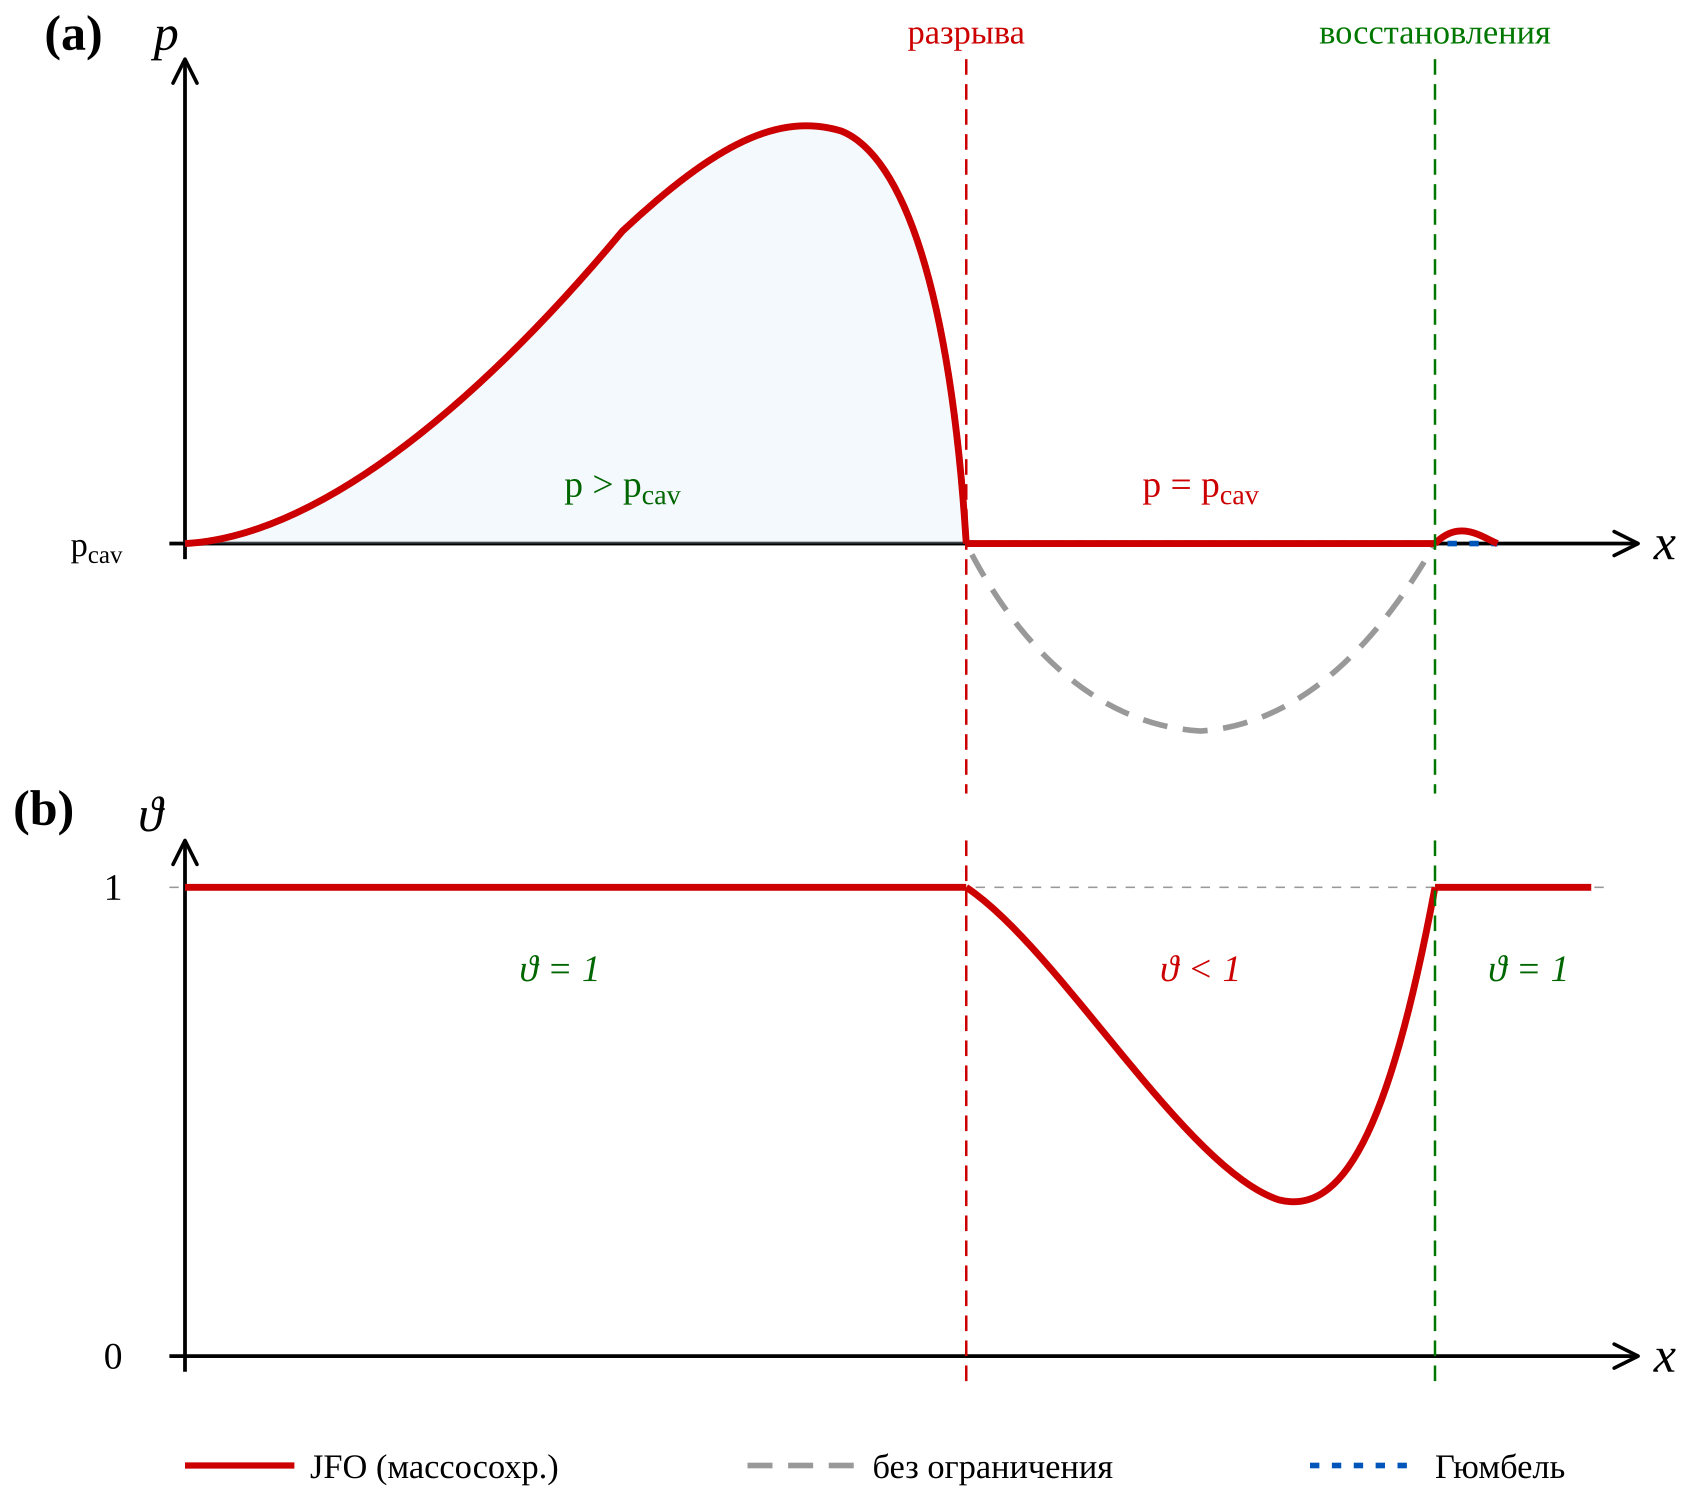
\includegraphics[width=\textwidth,height=0.9\textheight,keepaspectratio]{figures/ch02/fig_2_19.png}
\caption{Сравнение моделей кавитации: обнуление давления (Гюмбель)
  и массосохраняющая постановка (JFO)}
\label{fig:jfo_1d_profile}
\end{figure}

%% Блок 4: Граничные условия
Граничные условия для давления задаются так же, как в
подразделах~2.1.2-2.1.4 (периодичность, заданное давление на входе
и~выходе).  На границах подачи смазки полагают $\vartheta = 1$
(полное заполнение).  По периодическим направлениям~$\vartheta$
подчиняется тем же условиям периодичности, что и~$p$.

%% Блок 5: Подводка к численной реализации
Задача~\eqref{eq:jfo_conservation}-\eqref{eq:jfo_complementarity}
является нелинейной задачей с неравенствами (комплементарность).
На практике её решают итерационно: на каждой итерации определяется
активное множество кавитации и полного заполнения, после чего
обновляются $p$ и $\vartheta$ при выполнении условий комплементарности.
Сравнение моделей кавитации (обнуление давления и JFO) на одномерном профиле давления иллюстрирует рис.~\ref{fig:jfo_1d_profile}. Численная схема дискретизации и алгоритм итерационного решения
приводятся в подразделе~2.3.3~\cite{elrod1975}.
